\documentclass[conference]{IEEEtran}
\IEEEoverridecommandlockouts
% The preceding line is only needed to identify funding in the first footnote. If that is unneeded, please comment it out.
\usepackage{amsmath,amsthm,amssymb} %modos matemáticos y  simbolos
\usepackage{latexsym,amsfonts} %simbolos matematicos
\usepackage{cancel} %hacer la linea que cancela las ecuaciones
\usepackage[spanish, es-noshorthands]{babel} %comandos en español y cambia el cuadro por la tabla
\decimalpoint %cambia las comas por puntos decimal
\usepackage[utf8]{inputenc} %caracteristicas del español
\usepackage{physics} %Simbolos fisicos
\usepackage{array} %mejores formatos de tabla
\parindent =0cm %sangria 
\usepackage{algorithmic}
\usepackage{graphicx}
\usepackage{textcomp}
\usepackage{xcolor}
\usepackage{mathtools} 
\usepackage[framemethod=TikZ]{mdframed}%Entornos talegas
\usepackage[colorlinks = true,
			linkcolor = blue,
			citecolor = black,
			urlcolor = blue]{hyperref}%formato de los links y URL's
\usepackage{multicol} %varias columnas
\usepackage{enumerate} %enumeraciones
\usepackage{pgf,tikz,pgfplots} %documentos en formato tikz
\usepackage{mathrsfs} %letras chingonas (transformada de laplace)
\usepackage{subfigure} %varias figuras seguidas
\usepackage{tabulary}
\usepackage{multirow} %ocupar varias filas en una tabla
\usepackage{fancybox} %recuadros talegas
\usepackage{float} %ubicar graficas
\usepackage{color}
\usepackage{comment}
\usepackage{stackrel}
\usepackage{calligra}
\usepackage{lipsum}
\usepackage{cite}
\pgfplotsset{compat=1.16} 

\newcommand{\R}{\mathbb{R}}
\newcommand{\Z}{\mathbb{Z}}
%%%%%%%%%%%%%%%%%%%%%%%%%%%%%%%%%%%%%%%%%%%%%%%%%%%%%%
\def\BibTeX{{\rm B\kern-.05em{\sc i\kern-.025em b}\kern-.08em
    T\kern-.1667em\lower.7ex\hbox{E}\kern-.125emX}}
\begin{document}

\title{Vida Media del Muón \\
{\footnotesize \scshape{Reporte 1}}
}

\author{\IEEEauthorblockN{1\textsuperscript{st} Diego Sarceño Ramírez}
\IEEEauthorblockA{\textit{201900109} 
}
%\and
%\IEEEauthorblockN{2\textsuperscript{nd} Andrés Pérez}
%\IEEEauthorblockA{\textit{201704199}
%}
%\and
%\IEEEauthorblockN{3\textsuperscript{rd} Diego Sarceño Ramírez}
%\IEEEauthorblockA{\textit{201900109} \\
%}
}



\maketitle

\begin{abstract}
    Se utilizaron los datos de un detector Cherenkov para encontrar pulsos dobles en cada uno de los eventos y aproximar el valor de la vida media de un muón. Para esta aproximación se utilizó un \textit{threshold} de $\mathbf{-800}$ para evitar el ruido y tener suficientes datos para el ajuste a una función exponencial.
\end{abstract}

\begin{IEEEkeywords}
	Cherenkov, root, histogramas, vida media, muón.
\end{IEEEkeywords}

%\section{Objetivos}
%
%\subsection{General}
%    \begin{enumerate}[1.]
%        \item Realizar un circuito sumador/restador de 3 bits de entrada con una salida de resultado en un display de 7 segmentos en formato base 10.
%    \end{enumerate}
%\subsection{Específicos}
%    \begin{enumerate}
%        \item Diseñar múltiples circuitos combinacionales para obtener un resultado único en conjunto.
%        \item Implementar un circuito de lógica combinacional capaz de realizar operaciones aritméticas simples utilizando únicamente compuertas lógicas.
%        \item Optimizar el uso de compuertas mediante técnicas distintas al uso de Mapas de Karnaugh.
%        \item Contrastar los diseños teóricos con los resultados experimentales de los circuitos implementados físicamente.
%    \end{enumerate}
%\section{Introducción}
    
\section{Marco Teórico}
    La radiación Cherenkov es un fenómeno que ocurre cuando partículas cargadas atraviezan un material en el cual la luz viaja más lento. Esto genera una "Onda de Choque" en forma de polarización y luz ultravioleta. Esta señal llega a los fotoreceptores que, por ley de Ohm, generan una corriente y voltaje que es posible medirse. Esos voltajes medidos a un 'ratio'/frecuencia constante son los datos proporcionados en los archivos \texttt{.paa}. Para que el medidor se active e inicie a la medición del evento, es necesario un voltaje de \textit{threshold}, en este caso es $-150$, mientras que para detectar los pulsos dobles, nosotros usaremos $-800$ de threshold, con esto es suficiente para generar un buen conjunto de datos. \\
    
   Este conjunto de datos se ajustará a una función exponencial gracias a la teoría de la desintegración, obedeciendo la siguiente ecuación
	$$N(t) = N_o e^{-\lambda t}$$
%\section{Diseño Experimental}



\section{Montaje Experimental}
%    \subsection{Materiales a Utilizar}
%        \begin{itemize}
%    	\item 
%    \end{itemize}
%
%    \subsection{Procedimientos}
%        \begin{enumerate}
%            \item 
%        \end{enumerate}

Para este experimento se utilizó como guía el \textit{script} proporcionado por el catedrático al cual se le realizaron ciertos cambios. Se agregan 3 condicionales \texttt{if}, dado que lo que buscamos es tener únicamente los pulsos dobles, eliminamos el primer pulso del evento (al igual que los puntos cercanos, acotamos esto a una marca de tiempo menor a $20$) y nombramos una variable contador en $1$. Al seguir en el mismo evento, se establece el nuevo \textit{Threshold} en $-800$ y una marca de tiempo mayor a $100$, esto para evitar tomar datos de ruido. Y el tercer \texttt{if} muestra los datos en pantalla. \\

Con esto se crea un \textit{script} que plotea el histograma y realiza el ajuste exponencial ("expo"). Con esto se obtienen las gráficas mostradas en resultados. Los códigos pueden ser encontrados junto con este \texttt{.pdf} o en el siguiente \href{https://github.com/DSarceno/Semestre9/blob/master/Laboratorio\%20Avanzado/Vida_media_muon/Codigos}{GitHub}\footnote{El archivo de lectura es el llamado \texttt{modReadPAA.C} y el que realiza el histograma es el archivo \texttt{hist.C}.}.
        
        
        
        
\section{Resultados}
    Las gráficas se muestran en la sección de anexos. El valor real de la vida media del muón es $2.2\mu s$, se compararan los valores encontrados por el ajuste exponencial con el valor real. La escala de tiempo es de $8ns$.
    \begin{table}[H]
    	\centering
    	\caption{Tabla de tiempos (Vida Media del Muon)}
		\label{table:tiempos}
		\begin{tabular}{||c||c|c|c||}
			\hline
			\hline
			File & Media $\pm$ Std   & $t\pm \Delta t\, [\mu s]$ & $\% E$      \\
			\hline
			\hline
			$1$    & $355.6 \pm 218.5$ & $2.84 \pm 1.75$         & $29\%$    \\
			$2$    & $347.4 \pm 201.8$ & $2.78\pm 1.61$          & $26.3\%$  \\
			$3$    & $387.5 \pm 244.5$ & $3.1\pm 1.96$           & $40.9\%$  \\
			$4$    & $410.3\pm 238.6$  & $3.28\pm 1.91$          & $49\%$    \\
			$5$    & $410.2\pm 226.9$  & $3.28\pm 1.82$          & $49\%$    \\
			$6$    & $331.6\pm 205.7$  & $2.65\pm 1.64$          & $20.45\%$ \\
			\hline
			\hline
		\end{tabular}
	\end{table}
    
    
    
\section{Discusión de Resultados}
\begin{enumerate}
    \item Al ver la tabla \ref{table:tiempos}, podemos ver claramente un error bastante grande respecto al valor real de la vida media del muón. Esto puede ser por varias razones: el experimento en sí, la calidad de los datos o el \textit{threshold} que se utilizó para acotar y seleccionar bien bien los pulsos dobles. 
    \item Como se mencionó, se escogió este \textit{threshold} para evitar a toda costa los datos de ruido y que fuera más eficiente el código, esto pudo causar cierto aumento en el error; sin embargo, la gráfica \ref{fig:file6}, \ref{fig:file2} y \ref{fig:file1} son las que más se asemejan (a la vista) a una exponencial y por ende, son las que presentan menor error.
	\item Para las gráficas \ref{fig:file4} y \ref{fig:file5} que presentan datos un poco desproporcionados, se puede ver gráficamente que son datos aislados los que se escapan de la distribución.
	\item Mientras que la gráfica \ref{fig:file5} presenta datos desproporcionados, estos no son justificables y puede pertenecer a alguna de las razones mencionadas en el primer inciso de esta sección.
\end{enumerate}



\section{Conclusiones}
\begin{enumerate}
    \item El efecto Cherenkov es viable para aproximar el valor medio de partículas cargadas; sin embargo, es necesario un buen equipo para evitar el ruido y un buen \textit{threshold} que nos permita suficientes datos para aproximar el valor pero evite los datos de ruido.
\end{enumerate}
%\section{Recomendaciones}

\section{Anexos}
		\begin{figure}[H]
            \centering
            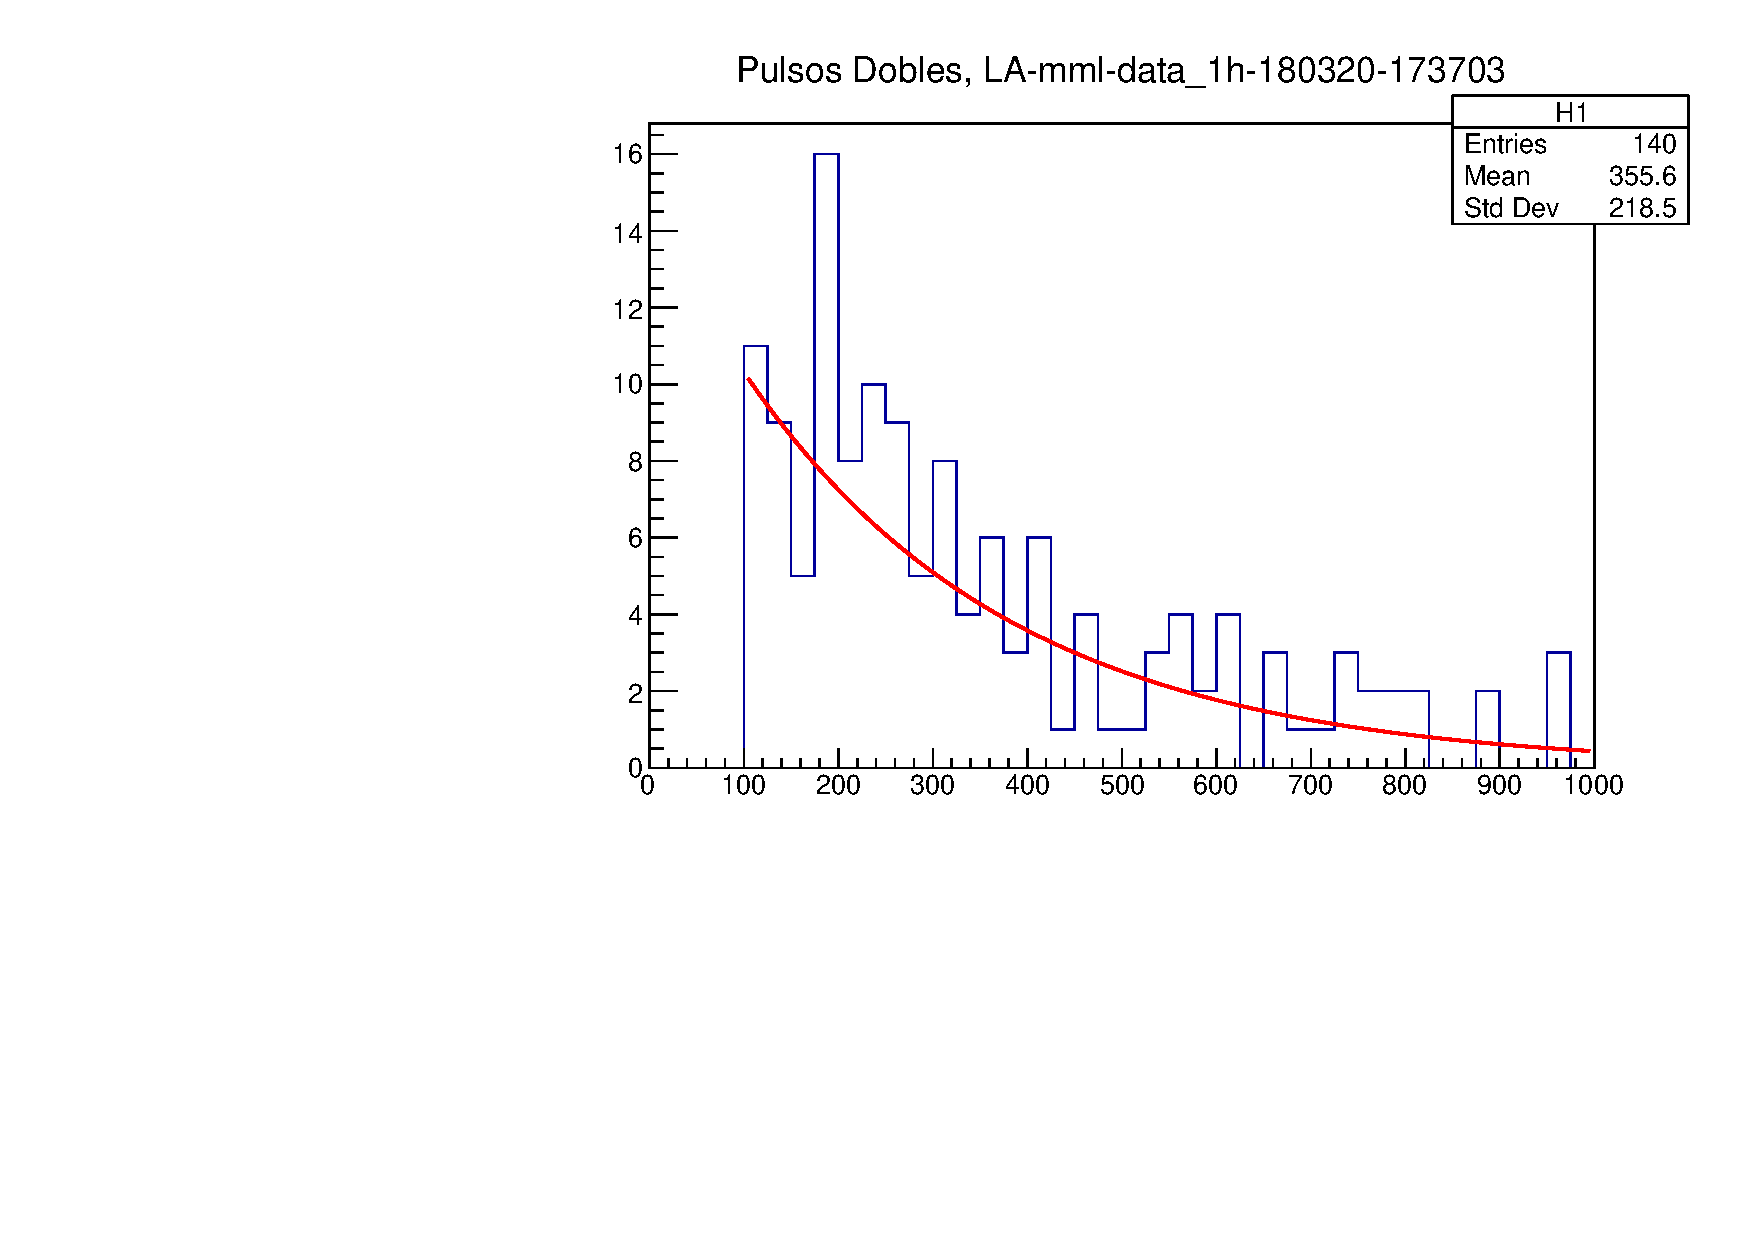
\includegraphics[scale=0.4]{./Imagenes/file1.pdf}
            \caption{Histograma del archivo de datos terminado en: $173703$}
            \label{fig:file1}
        \end{figure}  
        \begin{figure}[H]
            \centering
            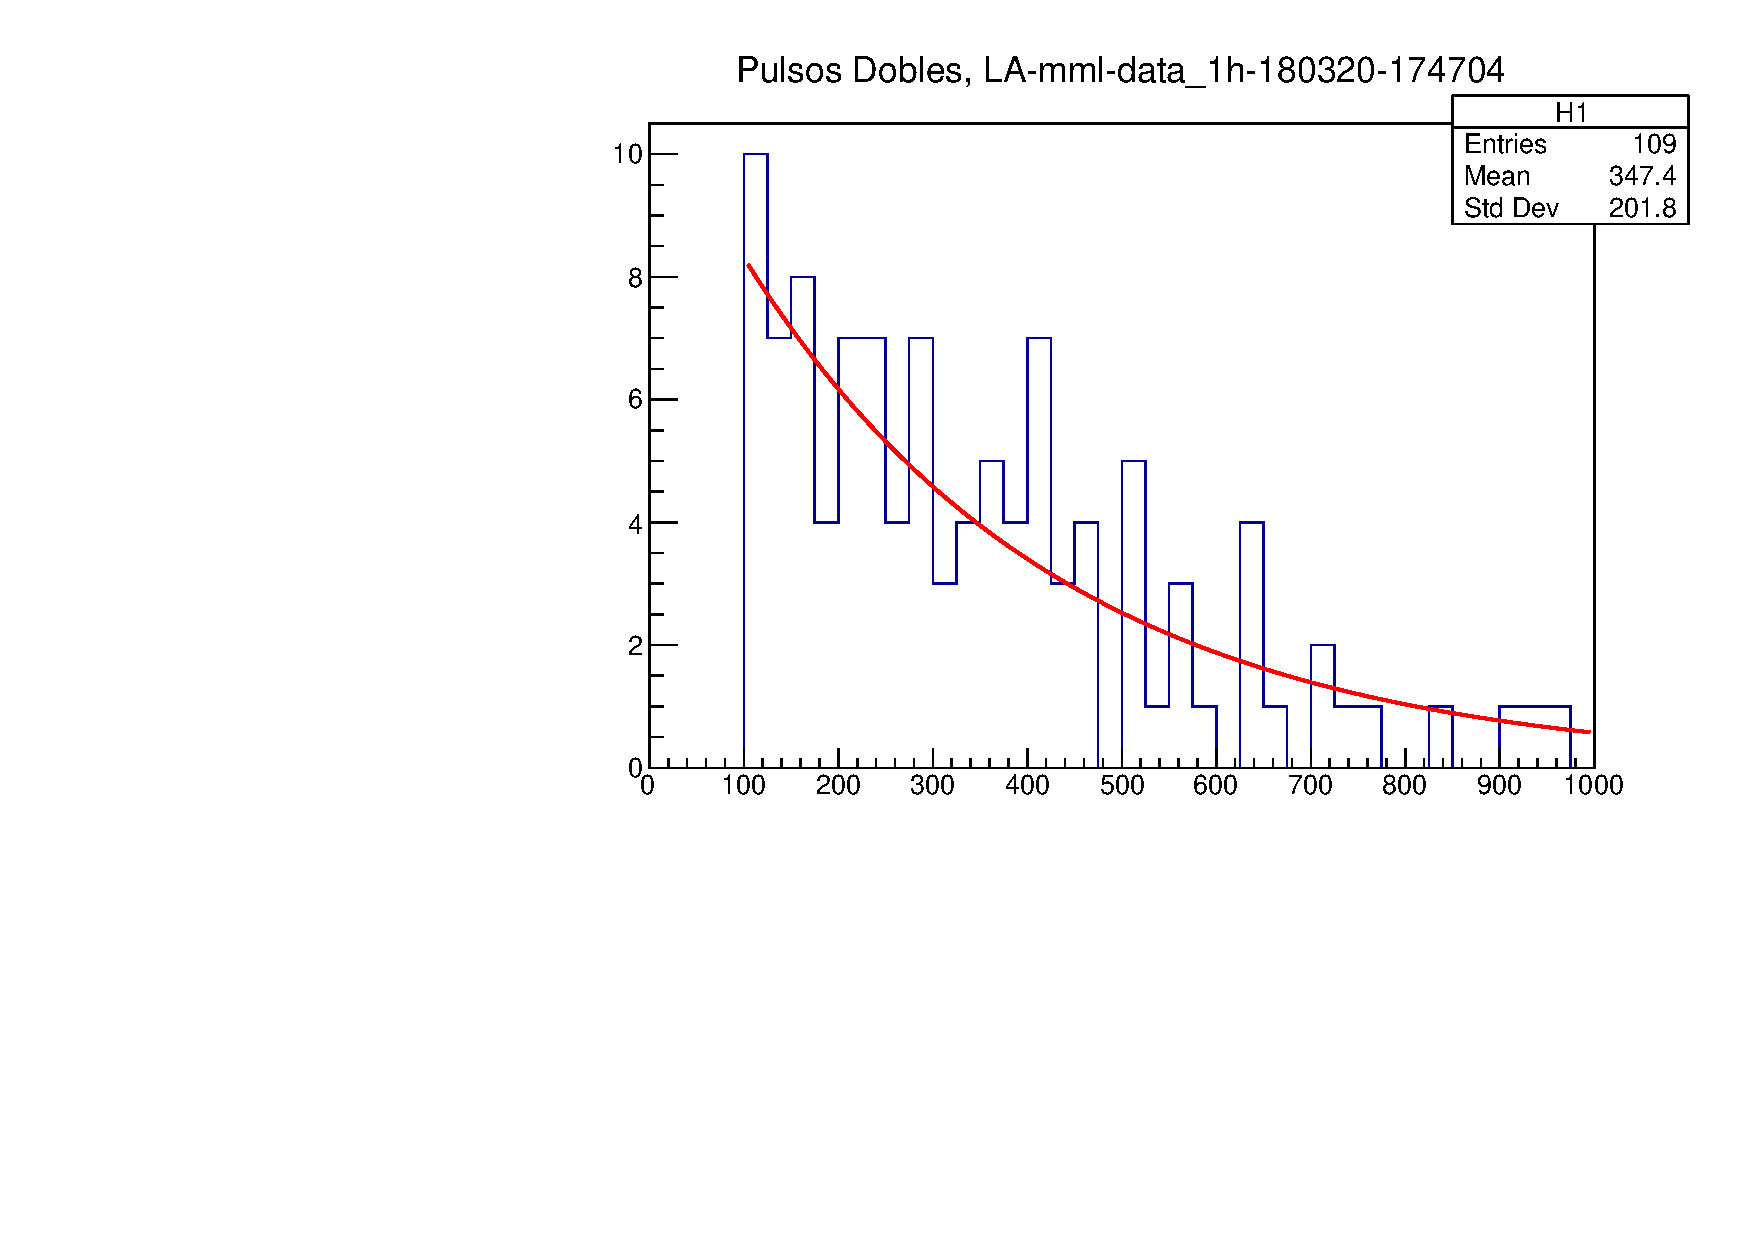
\includegraphics[scale=0.4]{./Imagenes/file2.pdf}
            \caption{Histograma del archivo de datos terminado en: $174704$}
            \label{fig:file2}
        \end{figure} 
        \begin{figure}[H]
            \centering
            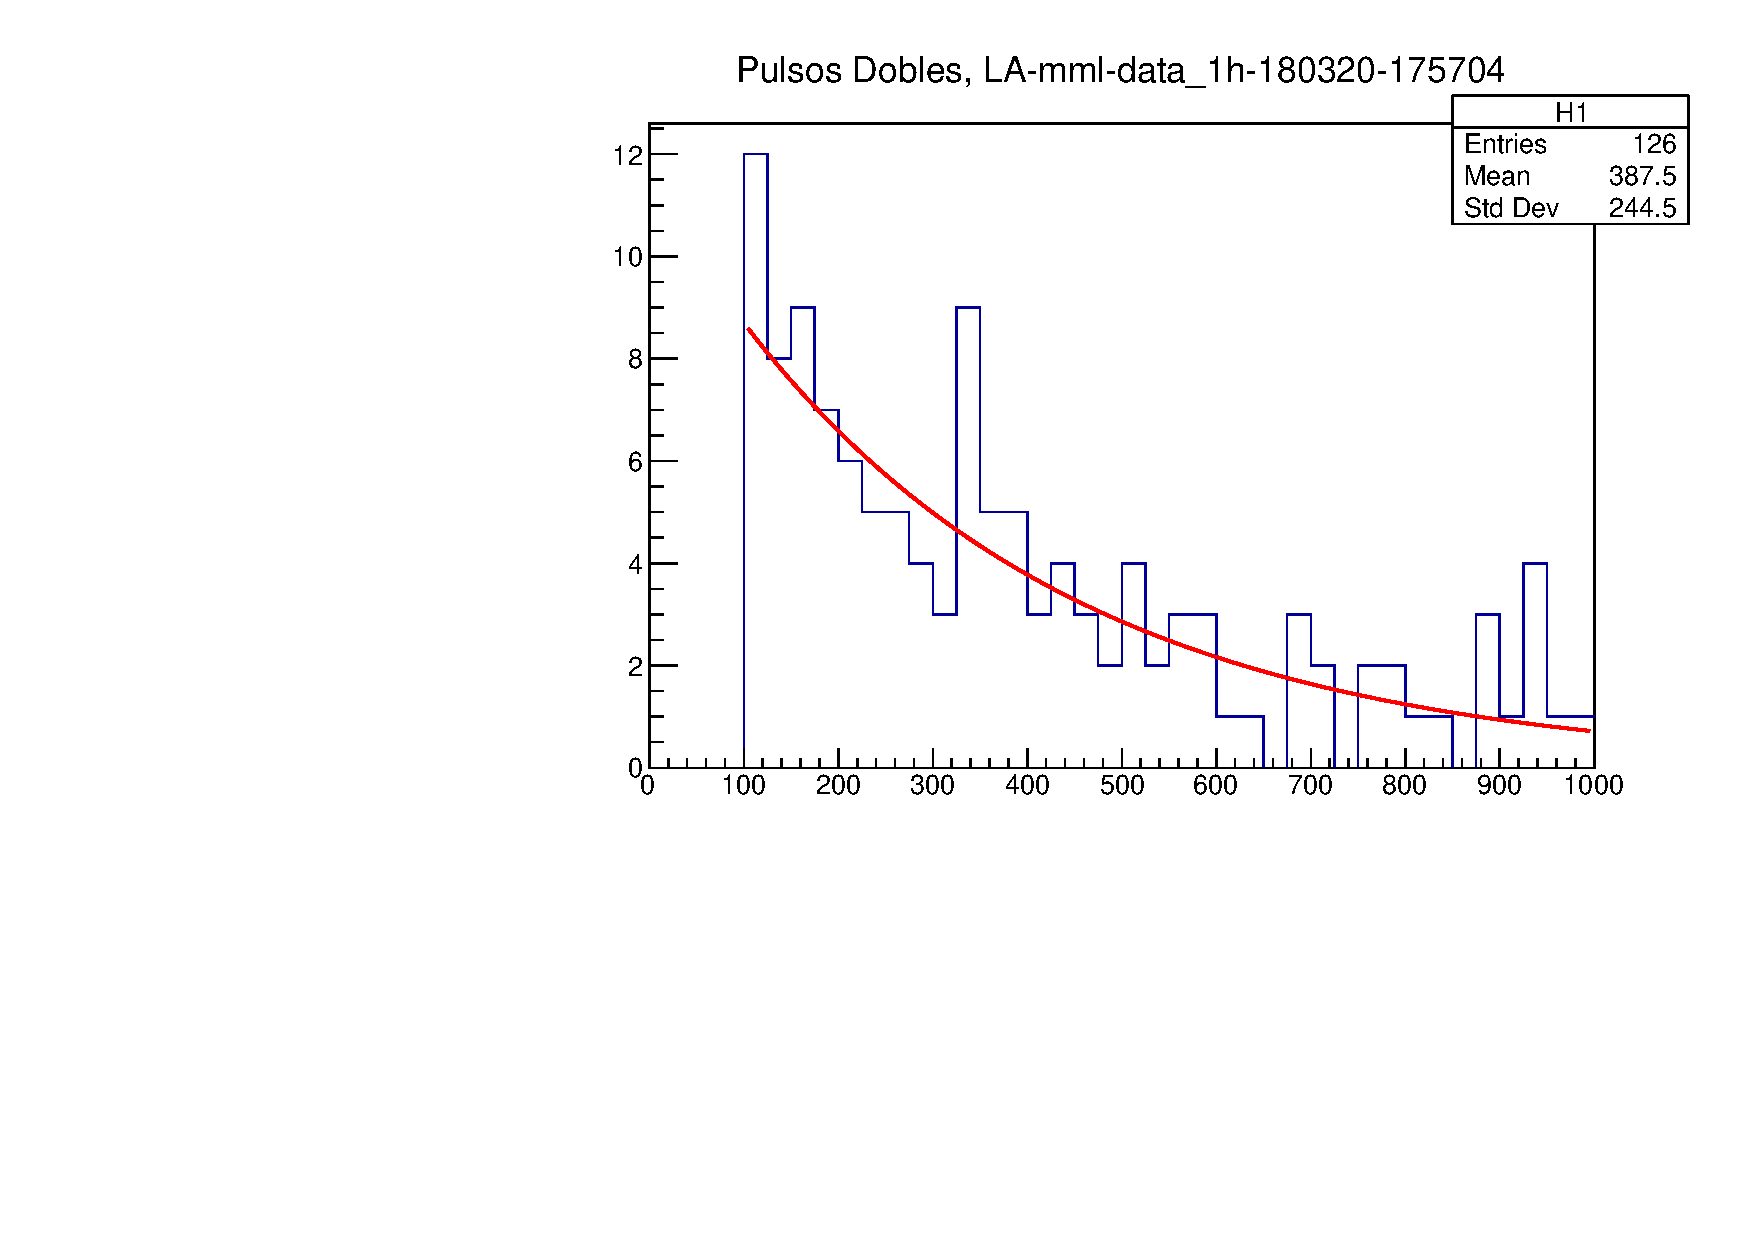
\includegraphics[scale=0.4]{./Imagenes/file3.pdf}
            \caption{Histograma del archivo de datos terminado en: $175704$}
            \label{fig:file3}
        \end{figure}  
        \begin{figure}[H]
            \centering
            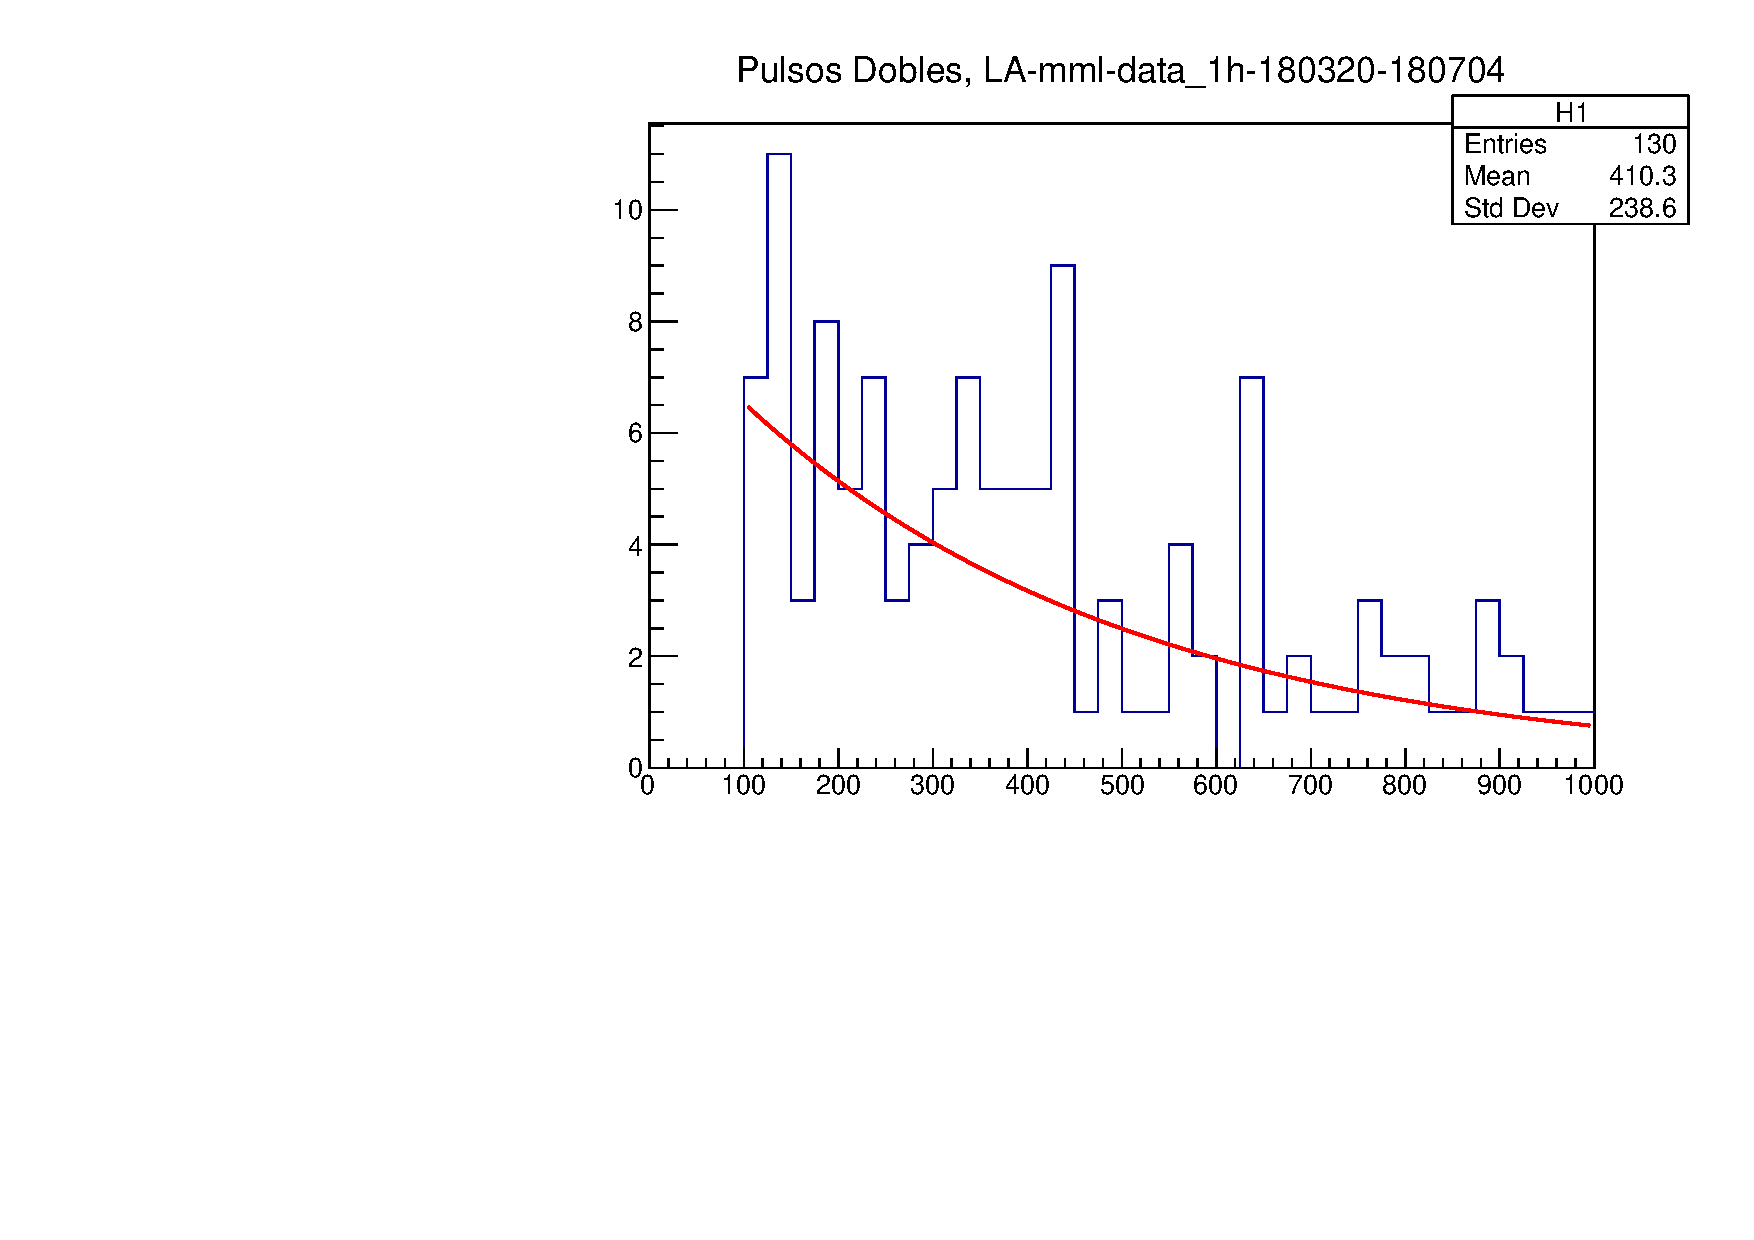
\includegraphics[scale=0.4]{./Imagenes/file4.pdf}
            \caption{Histograma del archivo de datos terminado en: $180704$}
            \label{fig:file4}
         \end{figure} 
         \begin{figure}[H]
            \centering
            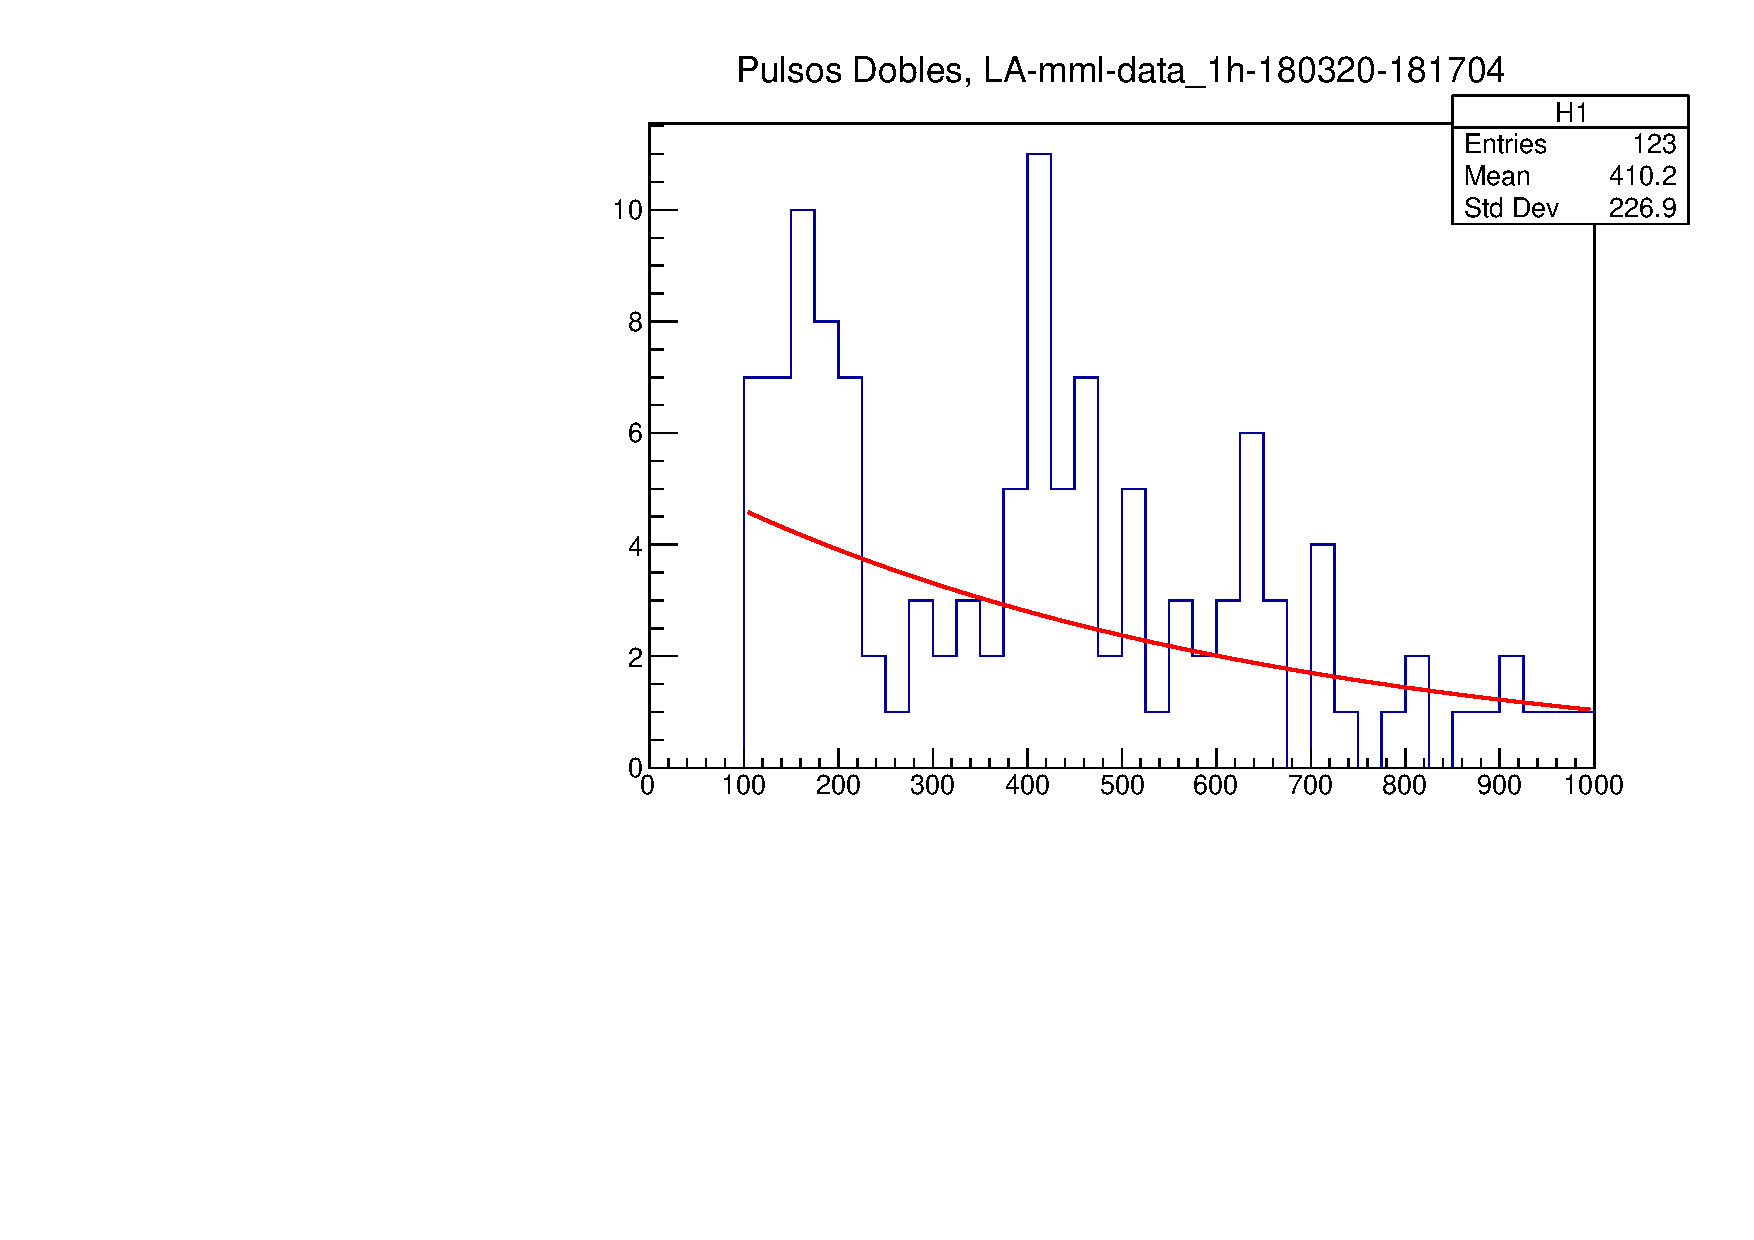
\includegraphics[scale=0.4]{./Imagenes/file5.pdf}
            \caption{Histograma del archivo de datos terminado en: $181704$}
            \label{fig:file5}
         \end{figure} 
         \begin{figure}[H]
            \centering
            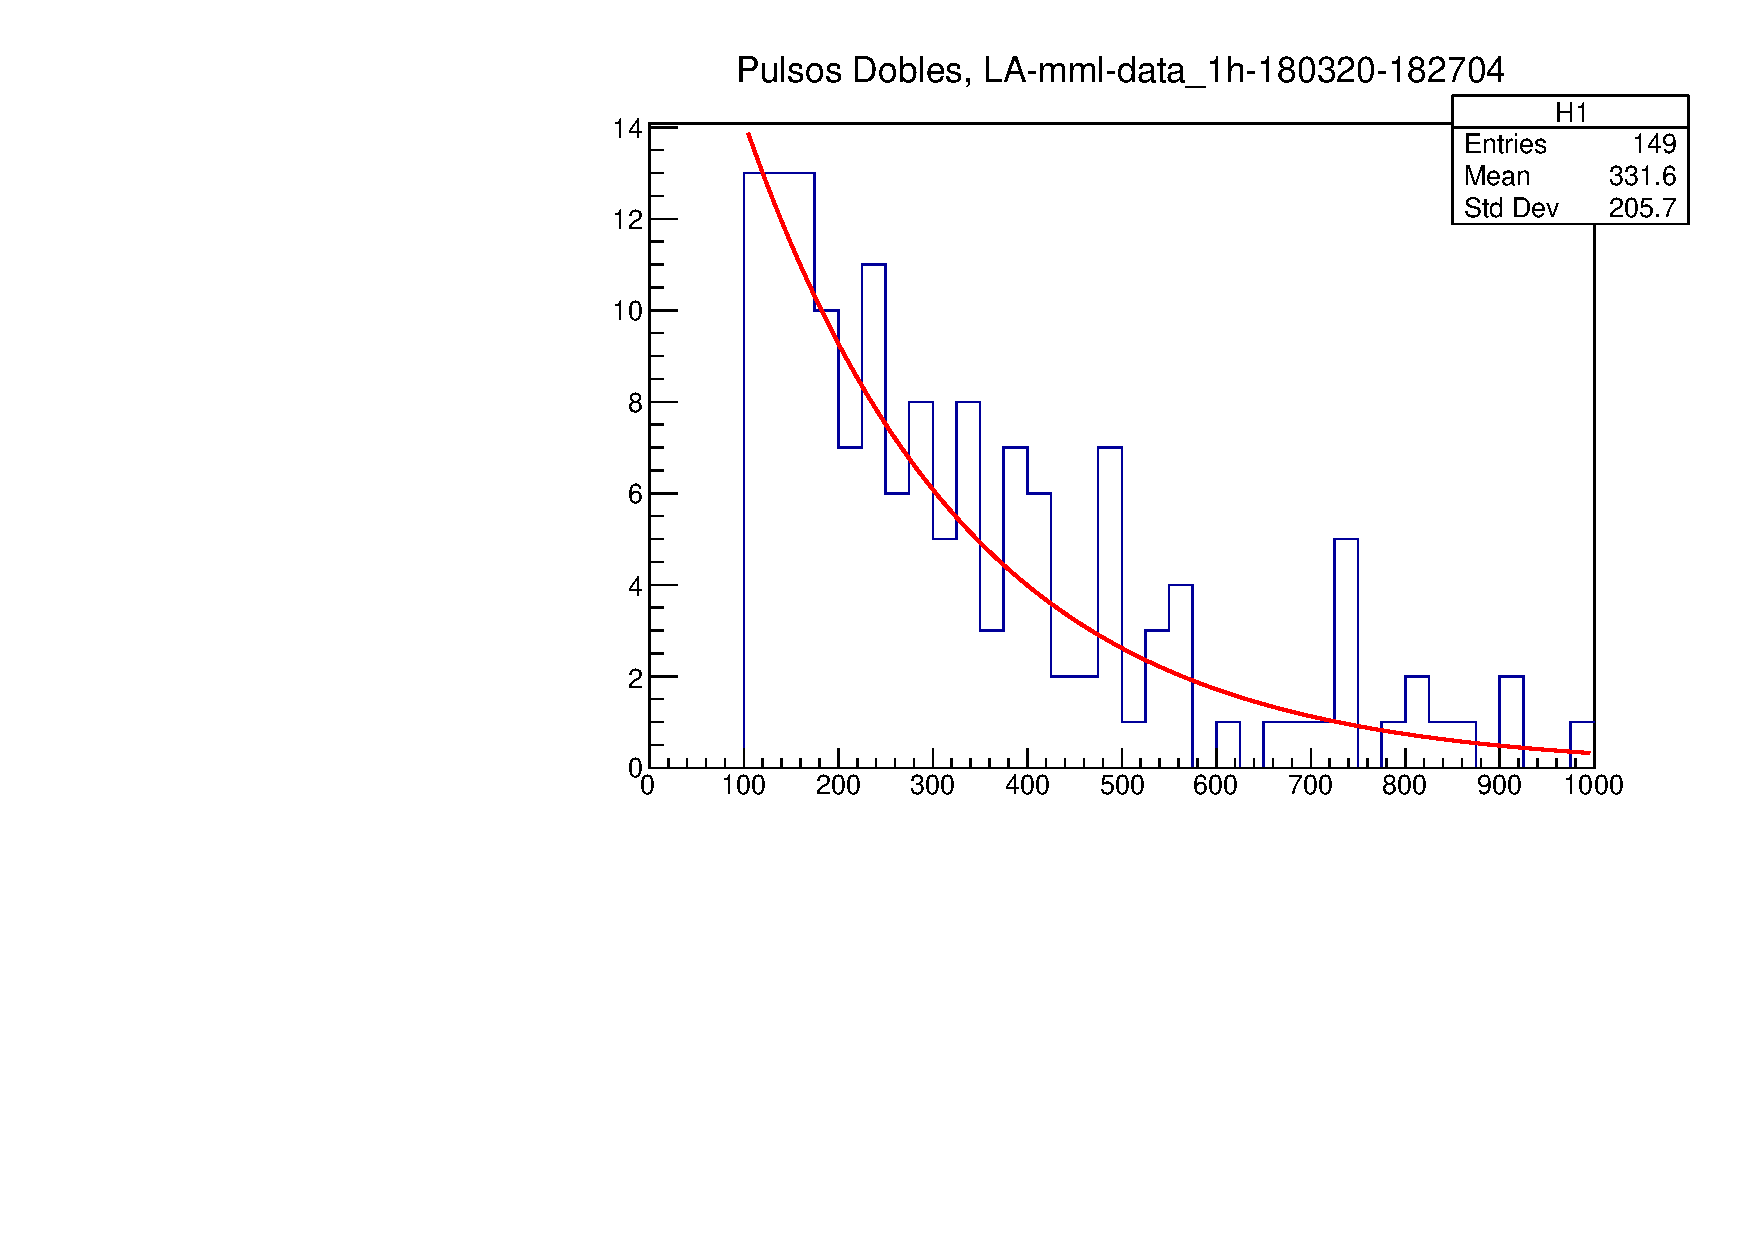
\includegraphics[scale=0.4]{./Imagenes/file6.pdf}
            \caption{Histograma del archivo de datos terminado en: $182704$}
            \label{fig:file6}
         \end{figure} 
        
        
        
        
\begin{thebibliography}{00}
\bibitem{b2} \textit{Chapter: Histograms}. \url{https://root.cern.ch/root/htmldoc/guides/users-guide/Histograms.html}
\end{thebibliography}

\end{document}


